%%%%%%%%%%%%%%%%%%%%%%%%%%%%%%%%%%%%%%%%%%%%%%%%%%%%%%
%% Master Thesis, LaTeX Template                    %%
%% Copyleft by Piotr Wozniak & Artur M. Brodzki     %%
%% Faculty of Electronic and Information Technology %%
%% Warsaw University of Technology, Warsaw, 2019    %%
%%%%%%%%%%%%%%%%%%%%%%%%%%%%%%%%%%%%%%%%%%%%%%%%%%%%%%

\documentclass{eiti/eiti-mgr}

%\usepackage{fontspec} %custom fonts
\usepackage[polish]{babel}

%alternatywne czcionki 
%\setmainfont{Adagio Slab}
%\setromanfont{times.ttf}
%\setsansfont{arial.ttf}

\begin{document}

%--------------------------------
% Strona tytułowa
%--------------------------------
\instytut{XXXXXX}
\kierunek{XXXXXX}
\specjalnosc{XXXXXX}
\title{Niepotrzebnie długi i skomplikowany tytuł pracy \\ trudny do przeczytania, zrozumienia i wymówienia}
\author{XXXXXX}
\album{XXXXXX}
\promotor{XXXXXX}
\date{\the\year}
\maketitle

%--------------------------------
% Streszczenie po polsku
%--------------------------------
\streszczenie \lipsum[1-3]
\slowakluczowe XXX, XXX, XXX
\newpage

%--------------------------------
% Streszczenie po angielsku
%--------------------------------
\abstract \kant[1-3]
\keywords XXX, XXX, XXX
\newpage

%--------------------------------
% Oświadczenie o autorstwie
%--------------------------------
\makeauthorship
\newpage

%--------------------------------
% Spis treści
%--------------------------------
\thispagestyle{plain}
\tableofcontents
\newpage

%--------------------------------
% Rozdziały
%--------------------------------

\section{Wstęp}
\lipsum[1-2] \cite{greenwade93}
\begin{figure}[h]
	\label{fig:anzelm}
	\centering 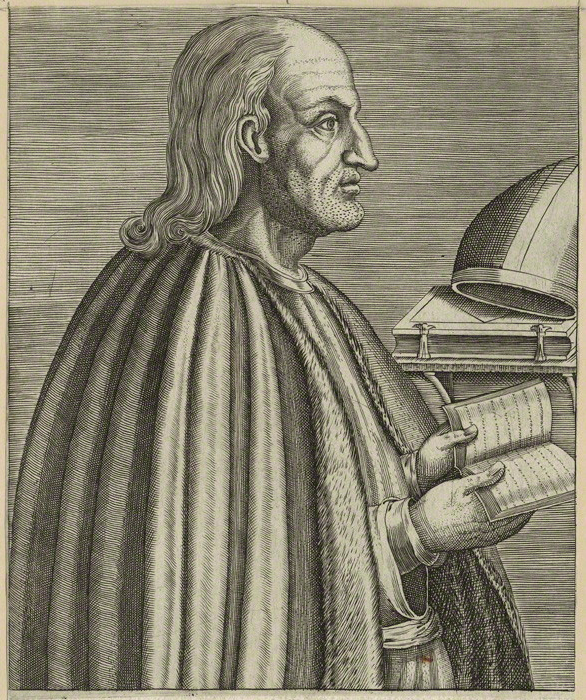
\includegraphics[width=0.7\linewidth]{img/anzelm.png}
	\caption{Anzelm z Canterbury.}
\end{figure}
\lipsum[3-4]

\section{De Finibus Bonorum et Malorum}
\lipsum[1-2]

\begin{align*}
	E & = mc^2 \\ 
	y & = ax^2 + bx + c
\end{align*}

\lipsum[3]

\begin{align}
\begin{bmatrix}
1 & 0 & 0 \\ 
0 & 2 & 0 \\ 
0 & 0 & 3
\end{bmatrix} \cdot 
\begin{bmatrix}
4 \\ 5 \\ 6
\end{bmatrix} = 
\begin{bmatrix}
4 \\ 10 \\ 18
\end{bmatrix}
\end{align}

\lipsum[4] \cite{goossens93}

\subsection{Critique of Pure Reason}
\kant[1]
\begin{table} \label{tab:tabela1} \centering
\begin{tabular} {| c | c | r |} \hline
	Kolumna 1 & Kolumna 2 & Liczba \\ \hline\hline
	cell1 & cell2 & 60 \\ \hline
	cell4 & cell5 & 43 \\ \hline
	cell7 & cell8 & 20,45 \\ \hline
	\multicolumn{2}{|r|}{Suma:} & 123,45 \\ \hline
\end{tabular} \caption{Przykładowa tabela.}
\end{table}
\kant[2-3]

\section{Podsumowanie}
\lipsum[5-8]

%--------------------------------
% Literarura
%--------------------------------
\newpage
\bibliographystyle{apalike}
\bibliography{literatura}

%--------------------------------
% Spisy
%--------------------------------
\newpage
\listoffigures
\newpage
\listoftables

\end{document}

